\PassOptionsToPackage{unicode=true}{hyperref} % options for packages loaded elsewhere
\PassOptionsToPackage{hyphens}{url}
%
\documentclass[
  ignorenonframetext,
]{beamer}
\usepackage{pgfpages}
\setbeamertemplate{caption}[numbered]
\setbeamertemplate{caption label separator}{: }
\setbeamercolor{caption name}{fg=normal text.fg}
\beamertemplatenavigationsymbolsempty
% Prevent slide breaks in the middle of a paragraph:
\widowpenalties 1 10000
\raggedbottom
\setbeamertemplate{part page}{
  \centering
  \begin{beamercolorbox}[sep=16pt,center]{part title}
    \usebeamerfont{part title}\insertpart\par
  \end{beamercolorbox}
}
\setbeamertemplate{section page}{
  \centering
  \begin{beamercolorbox}[sep=12pt,center]{part title}
    \usebeamerfont{section title}\insertsection\par
  \end{beamercolorbox}
}
\setbeamertemplate{subsection page}{
  \centering
  \begin{beamercolorbox}[sep=8pt,center]{part title}
    \usebeamerfont{subsection title}\insertsubsection\par
  \end{beamercolorbox}
}
\AtBeginPart{
  \frame{\partpage}
}
\AtBeginSection{
  \ifbibliography
  \else
    \frame{\sectionpage}
  \fi
}
\AtBeginSubsection{
  \frame{\subsectionpage}
}
\usepackage{lmodern}
\usepackage{amssymb,amsmath}
\usepackage{ifxetex,ifluatex}
\ifnum 0\ifxetex 1\fi\ifluatex 1\fi=0 % if pdftex
  \usepackage[T1]{fontenc}
  \usepackage[utf8]{inputenc}
  \usepackage{textcomp} % provides euro and other symbols
\else % if luatex or xelatex
  \usepackage{unicode-math}
  \defaultfontfeatures{Scale=MatchLowercase}
  \defaultfontfeatures[\rmfamily]{Ligatures=TeX,Scale=1}
\fi
% use upquote if available, for straight quotes in verbatim environments
\IfFileExists{upquote.sty}{\usepackage{upquote}}{}
\IfFileExists{microtype.sty}{% use microtype if available
  \usepackage[]{microtype}
  \UseMicrotypeSet[protrusion]{basicmath} % disable protrusion for tt fonts
}{}
\makeatletter
\@ifundefined{KOMAClassName}{% if non-KOMA class
  \IfFileExists{parskip.sty}{%
    \usepackage{parskip}
  }{% else
    \setlength{\parindent}{0pt}
    \setlength{\parskip}{6pt plus 2pt minus 1pt}}
}{% if KOMA class
  \KOMAoptions{parskip=half}}
\makeatother
\usepackage{xcolor}
\IfFileExists{xurl.sty}{\usepackage{xurl}}{} % add URL line breaks if available
\IfFileExists{bookmark.sty}{\usepackage{bookmark}}{\usepackage{hyperref}}
\hypersetup{
  pdftitle={Trabalho Final},
  pdfauthor={Gilmar Pereira, Maressa Tavares e Victor Ruela},
  pdfborder={0 0 0},
  breaklinks=true}
\urlstyle{same}  % don't use monospace font for urls
\newif\ifbibliography
\usepackage{color}
\usepackage{fancyvrb}
\newcommand{\VerbBar}{|}
\newcommand{\VERB}{\Verb[commandchars=\\\{\}]}
\DefineVerbatimEnvironment{Highlighting}{Verbatim}{commandchars=\\\{\}}
% Add ',fontsize=\small' for more characters per line
\usepackage{framed}
\definecolor{shadecolor}{RGB}{248,248,248}
\newenvironment{Shaded}{\begin{snugshade}}{\end{snugshade}}
\newcommand{\AlertTok}[1]{\textcolor[rgb]{0.94,0.16,0.16}{#1}}
\newcommand{\AnnotationTok}[1]{\textcolor[rgb]{0.56,0.35,0.01}{\textbf{\textit{#1}}}}
\newcommand{\AttributeTok}[1]{\textcolor[rgb]{0.77,0.63,0.00}{#1}}
\newcommand{\BaseNTok}[1]{\textcolor[rgb]{0.00,0.00,0.81}{#1}}
\newcommand{\BuiltInTok}[1]{#1}
\newcommand{\CharTok}[1]{\textcolor[rgb]{0.31,0.60,0.02}{#1}}
\newcommand{\CommentTok}[1]{\textcolor[rgb]{0.56,0.35,0.01}{\textit{#1}}}
\newcommand{\CommentVarTok}[1]{\textcolor[rgb]{0.56,0.35,0.01}{\textbf{\textit{#1}}}}
\newcommand{\ConstantTok}[1]{\textcolor[rgb]{0.00,0.00,0.00}{#1}}
\newcommand{\ControlFlowTok}[1]{\textcolor[rgb]{0.13,0.29,0.53}{\textbf{#1}}}
\newcommand{\DataTypeTok}[1]{\textcolor[rgb]{0.13,0.29,0.53}{#1}}
\newcommand{\DecValTok}[1]{\textcolor[rgb]{0.00,0.00,0.81}{#1}}
\newcommand{\DocumentationTok}[1]{\textcolor[rgb]{0.56,0.35,0.01}{\textbf{\textit{#1}}}}
\newcommand{\ErrorTok}[1]{\textcolor[rgb]{0.64,0.00,0.00}{\textbf{#1}}}
\newcommand{\ExtensionTok}[1]{#1}
\newcommand{\FloatTok}[1]{\textcolor[rgb]{0.00,0.00,0.81}{#1}}
\newcommand{\FunctionTok}[1]{\textcolor[rgb]{0.00,0.00,0.00}{#1}}
\newcommand{\ImportTok}[1]{#1}
\newcommand{\InformationTok}[1]{\textcolor[rgb]{0.56,0.35,0.01}{\textbf{\textit{#1}}}}
\newcommand{\KeywordTok}[1]{\textcolor[rgb]{0.13,0.29,0.53}{\textbf{#1}}}
\newcommand{\NormalTok}[1]{#1}
\newcommand{\OperatorTok}[1]{\textcolor[rgb]{0.81,0.36,0.00}{\textbf{#1}}}
\newcommand{\OtherTok}[1]{\textcolor[rgb]{0.56,0.35,0.01}{#1}}
\newcommand{\PreprocessorTok}[1]{\textcolor[rgb]{0.56,0.35,0.01}{\textit{#1}}}
\newcommand{\RegionMarkerTok}[1]{#1}
\newcommand{\SpecialCharTok}[1]{\textcolor[rgb]{0.00,0.00,0.00}{#1}}
\newcommand{\SpecialStringTok}[1]{\textcolor[rgb]{0.31,0.60,0.02}{#1}}
\newcommand{\StringTok}[1]{\textcolor[rgb]{0.31,0.60,0.02}{#1}}
\newcommand{\VariableTok}[1]{\textcolor[rgb]{0.00,0.00,0.00}{#1}}
\newcommand{\VerbatimStringTok}[1]{\textcolor[rgb]{0.31,0.60,0.02}{#1}}
\newcommand{\WarningTok}[1]{\textcolor[rgb]{0.56,0.35,0.01}{\textbf{\textit{#1}}}}
\setlength{\emergencystretch}{3em}  % prevent overfull lines
\providecommand{\tightlist}{%
  \setlength{\itemsep}{0pt}\setlength{\parskip}{0pt}}
\setcounter{secnumdepth}{-2}

% set default figure placement to htbp
\makeatletter
\def\fps@figure{htbp}
\makeatother


\title{Trabalho Final}
\author{Gilmar Pereira, Maressa Tavares e Victor Ruela}
\date{03 dezembro 2019}

\begin{document}
\frame{\titlepage}

\begin{frame}

\end{frame}

\begin{frame}{Agenda}
\protect\hypertarget{agenda}{}

\begin{itemize}
\tightlist
\item
  Introdução
\item
  Descrição dos Dados
\item
  Revisão de literatura
\item
  Planejamento do Experimento
\item
  Análise Exploratória
\item
  Validação das premissas
\item
  Resultados
\item
  Conclusão
\end{itemize}

\end{frame}

\begin{frame}{Introdução \textbar{} Rotas de produção de aço}
\protect\hypertarget{introducao-rotas-de-producao-de-aco}{}

\end{frame}

\begin{frame}{Introdução \textbar{} Processo do Forno Elétrico}
\protect\hypertarget{introducao-processo-do-forno-eletrico}{}

\end{frame}

\begin{frame}{Introdução \textbar{} Objetivo}
\protect\hypertarget{introducao-objetivo}{}

Análise do desempenho das turma de operários em relação ao consumo de
oxigênio no processo de produção do aço usando um forno elétrico.

\end{frame}

\begin{frame}{Descrição dos Dados}
\protect\hypertarget{descricao-dos-dados}{}

\begin{itemize}
\tightlist
\item
  Os dados consistem no consumo de oxigênio registrado no processo de
  produção de aço em um forno elétrico;
\item
  Dados - Janeiro e Outubro de 2019;
\item
  Cada instância representa uma execução independente do processo;
\item
  Instâncias consideradas como outliers (erros de medição, valores
  absurdos) foram removidas;
\item
  Os dados foram normalizados por uma constante aleatória, por questões
  de confidencialidade.
\end{itemize}

\begin{table}[H]
\centering
\begin{tabular}{l|l|l|r}
\hline
turma & material & mes & VarConsumo\_Quimica\\
\hline
1 & 2 & 10 & 3.506712\\
\hline
0 & 2 & 10 & 2.945758\\
\hline
1 & 2 & 10 & 3.456152\\
\hline
\end{tabular}
\end{table}

\end{frame}

\begin{frame}{Revisão de Literatura}
\protect\hypertarget{revisao-de-literatura}{}

\begin{itemize}
\item
  \textbf{Blocagem} - Usada para eliminar ruídos conhecidos e
  controláveis {[}1{]} - Será usada para retirar a Sazonalidade dos
  dados em relação aos meses;
\item
  \textbf{Experimento Fatorial} - Eficiente para estudo de efeitos de
  dois ou mais fatores {[}1{]} - Será usado para analisar os dois
  fatores material e turma, e a interação entre eles.
\end{itemize}

\end{frame}

\begin{frame}{Planejamento do Experimento \textbar{} Objetivo}
\protect\hypertarget{planejamento-do-experimento-objetivo}{}

O objetivo é comparar o desempenho de 4 turmas em relação ao consumo de
oxigênio do processo, considerando também 9 diferentes materiais (tipos
de aço) produzidos para a comparação.

\textbf{Experimento:}

Portanto, um \textbf{experimento fatorial} será realizado para os
fatores \textbf{Turma} e \textbf{Material}. Além disso, a blocagem será
realizada para o fator \textbf{Mês}, objetivando remover efeitos de
sazonalidade dos dados,

Desta forma, aplica-se o testa \textbf{ANOVA} utilizando um modelo
linear {[}2{]}.

\end{frame}

\begin{frame}{Planejamento do Experimento \textbar{} Modelo}
\protect\hypertarget{planejamento-do-experimento-modelo}{}

\[\begin{equation}y_{ijk} = \mu + \tau_i + \beta_j + (\tau\beta)_{ij} + \delta_k +  \epsilon_{ijk}  \end{equation}\]

Onde:

\(\mu\) : média geral;

\(\tau_i\) : efeito do fator turma \(i\);

\(\beta_j\) : efeito do fator material \(j\);

\((\tau\beta)_{ij}\) : efeito da iteração da turma \(i\) com o material
\(j\);

\(\delta_k\) : efeito da blocagem do mês;

\(\epsilon_{ijk}\) : residos.

\end{frame}

\begin{frame}{Planejamento do Experimento \textbar{} Hipóteses}
\protect\hypertarget{planejamento-do-experimento-hipoteses}{}

Fator Turma:
\[\begin{cases} H_0: \tau_{i} = 0, \forall i &\\H_1:\exists \tau_{i} \neq 0 \end{cases}\]

Fator Material:
\[\begin{cases} H_0: \beta_{j} = 0, \forall j &\\H_1:\exists \beta_{j} \neq 0 \end{cases}\]
Efeito de interação:
\[\begin{cases} H_0: (\tau\beta)_{ij} = 0, \forall i,j &\\H_1:\exists (\tau\beta)_{ij} \neq 0 \end{cases}\]

\end{frame}

\begin{frame}{Planejamento do Experimento \textbar{} Parâmetros
experimentais}
\protect\hypertarget{planejamento-do-experimento-parametros-experimentais}{}

\begin{itemize}
\tightlist
\item
  Significância desejada: \(\alpha = 0.05\).
\item
  Mínima diferença de importância prática (padronizada):
  \(d^* = \delta^*/\sigma = 0.3\)
\item
  Potência mínima desejada \(\pi = 1 - \beta = 0.8\)
\end{itemize}

O \(d^* = 0.3\) foi escolhido para detectar diferenças ``médias'' na
magnitude {[}3{]}.

\end{frame}

\begin{frame}{Planejamento do Experimento \textbar{} Cálculo do número
de amostras}
\protect\hypertarget{planejamento-do-experimento-calculo-do-numero-de-amostras}{}

\[ \frac{F_{(1- \alpha)}^{a-1}}{F_{\beta, \phi}^{ab(n-1)}} = 1\]

\begin{table}[H]
\centering
\begin{tabular}{r|r|r}
\hline
n & ratio & phi\\
\hline
14 & 1.9430308 & 5.670\\
\hline
17 & 1.6103641 & 6.885\\
\hline
20 & 1.3678672 & 8.100\\
\hline
23 & 1.1846083 & 9.315\\
\hline
26 & 1.0419592 & 10.530\\
\hline
\textcolor{red}{\textbf{29}} & \textcolor{red}{\textbf{0.9281759}} & \textcolor{red}{\textbf{11.745}}\\
\hline
32 & 0.8355488 & 12.960\\
\hline
\end{tabular}
\end{table}

\end{frame}

\begin{frame}[fragile]{Análise Exploratória}
\protect\hypertarget{analise-exploratoria}{}

Número de amostras

\begin{verbatim}
## $turma
## turma
##    0    1    2    3 
## 1062  920  988  972 
## 
## $material
## material
##    0    1    2    3    4    5    6    7   13 
##  645  310 1200  316  196  192  651  265  167 
## 
## $mes
## mes
##   1   2   3   4   5   6   7   8   9  10 
## 351 365 399 457 439 402 453 337 377 362 
## 
## $`turma:material`
##      material
## turma   0  1   2  3  4  5   6  7 13
##     0 187 92 307 89 60 29 153 78 67
##     1 113 78 310 87 57 55 154 42 24
##     2 167 68 253 71 46 56 201 81 45
##     3 178 72 330 69 33 52 143 64 31
\end{verbatim}

\end{frame}

\begin{frame}{Análise Exploratória}
\protect\hypertarget{analise-exploratoria-1}{}

\begin{center}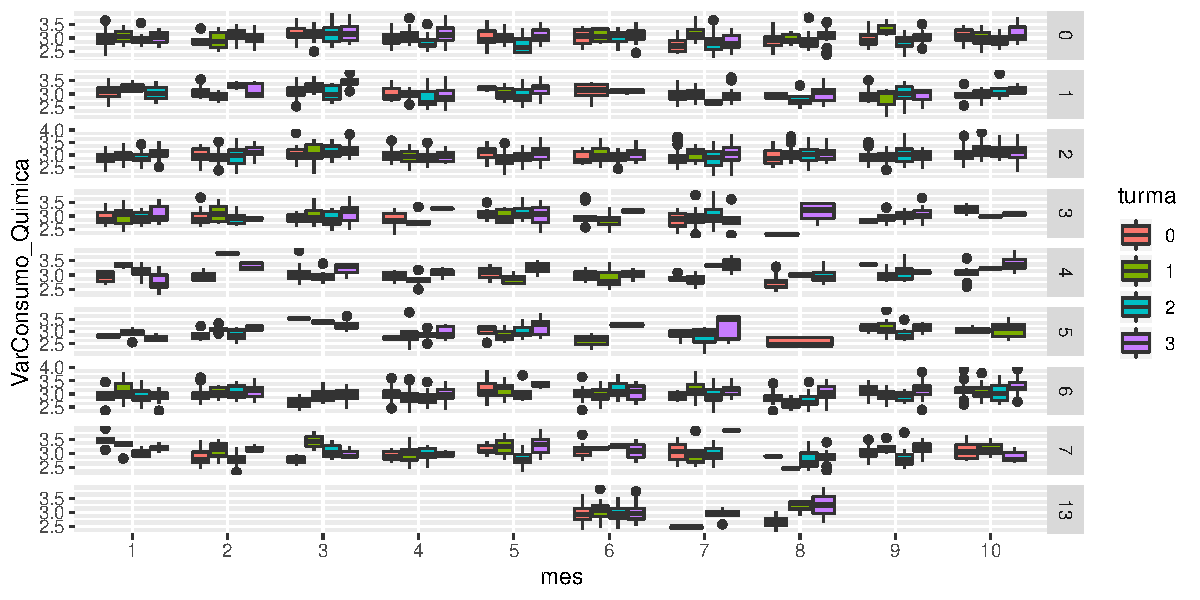
\includegraphics{apresentacao_final_files/figure-beamer/heat_count-1} \end{center}

O material 13 será removido por ter sido produzio somente em alguns
meses do ano.

\end{frame}

\begin{frame}{Análise Exploratória}
\protect\hypertarget{analise-exploratoria-2}{}

\begin{figure}

{\centering 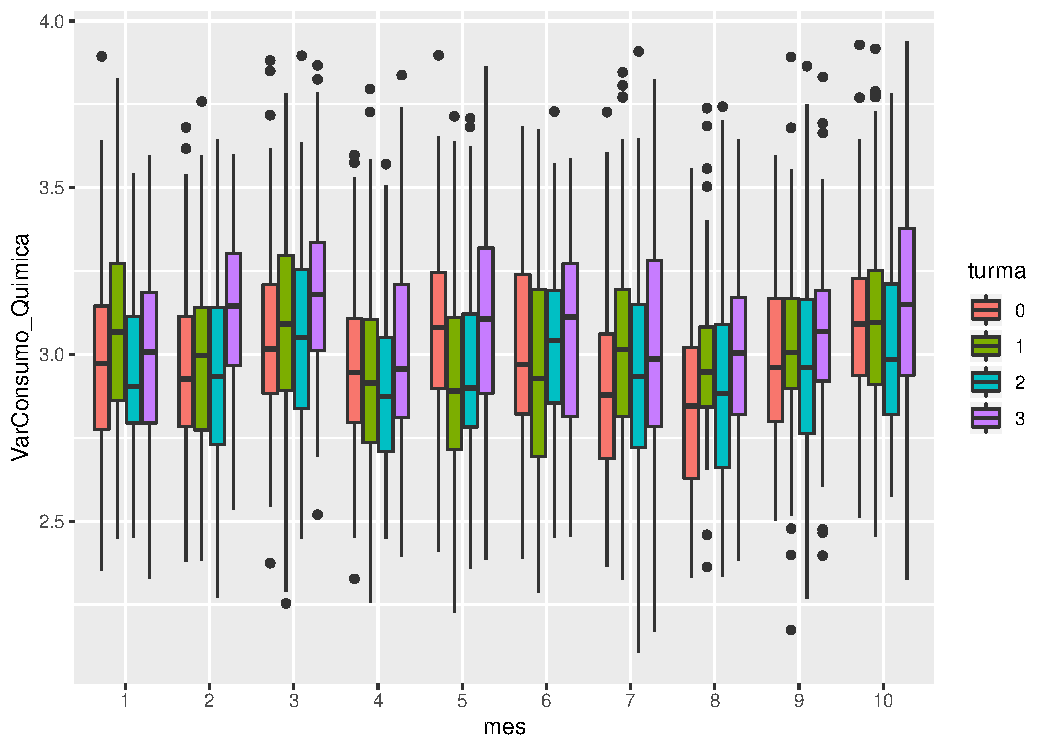
\includegraphics{apresentacao_final_files/figure-beamer/plot_eletrica-1} 

}

\caption{Boxplot da variável química}\label{fig:plot_eletrica}
\end{figure}

\end{frame}

\begin{frame}{Validação das premissas \textbar{} Normalidade}
\protect\hypertarget{validacao-das-premissas-normalidade}{}

Teste de Shapiro-Wilk - p-valor = \ensuremath{3.1376736\times 10^{-9}}

\begin{figure}

{\centering 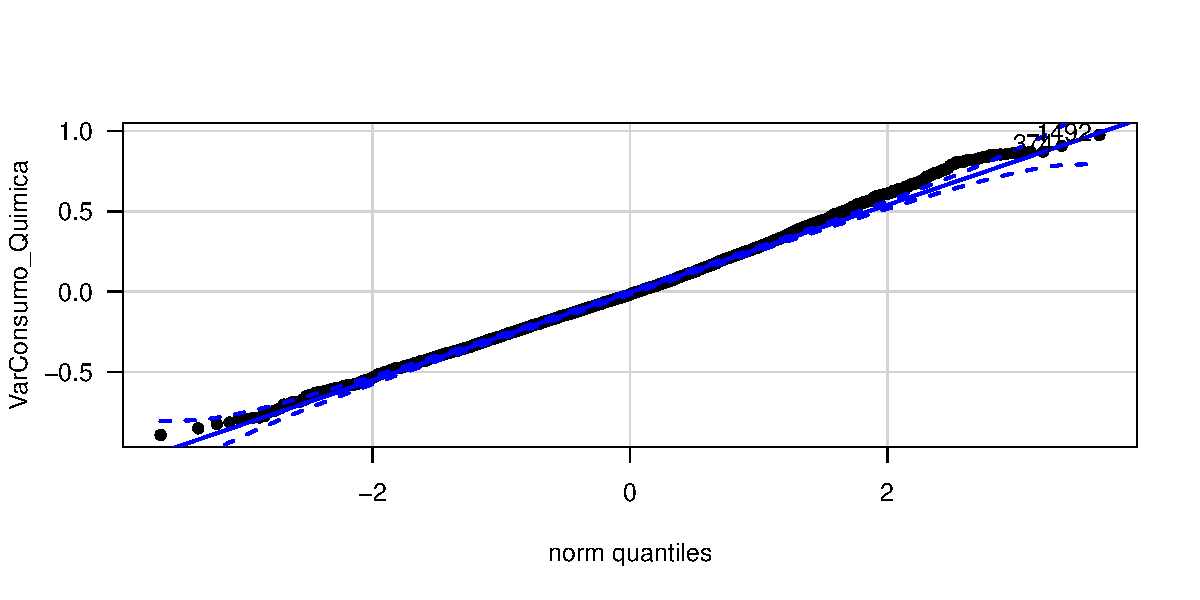
\includegraphics{apresentacao_final_files/figure-beamer/assum_norm-1} 

}

\caption{QQ plot para resíduos}\label{fig:assum_norm}
\end{figure}

\end{frame}

\begin{frame}{Validação das premissas \textbar{} Normalidade}
\protect\hypertarget{validacao-das-premissas-normalidade-1}{}

Teste de Shapiro-Wilk (transformação logarítmica) - p-valor = 0.0823771

\begin{figure}

{\centering 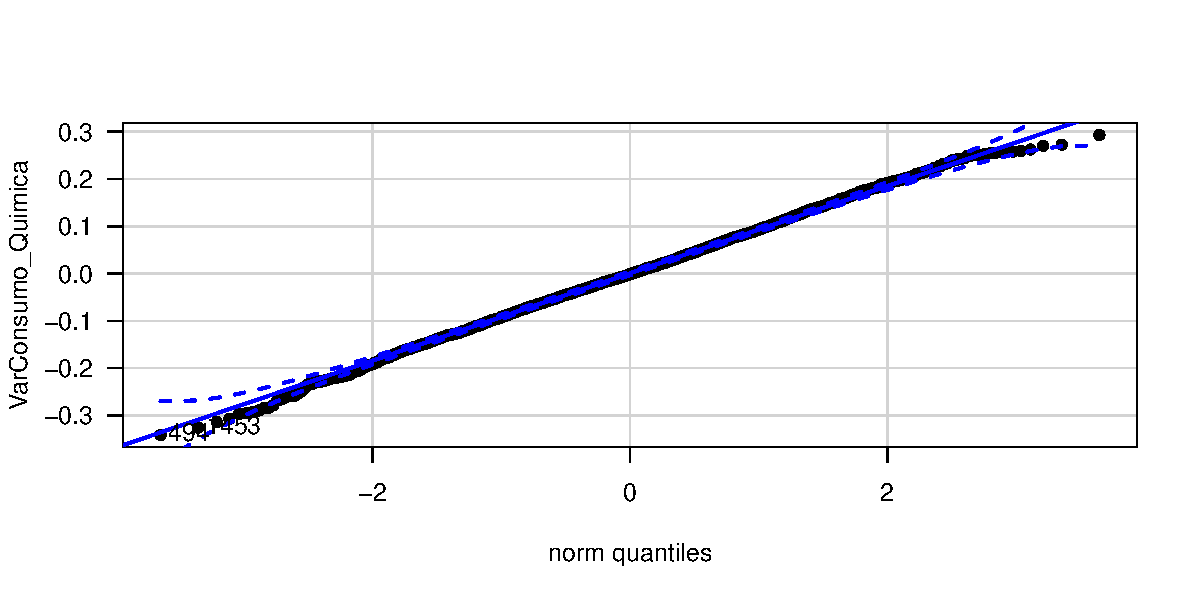
\includegraphics{apresentacao_final_files/figure-beamer/assum_norm_log-1} 

}

\caption{QQ plot para resíduos}\label{fig:assum_norm_log}
\end{figure}

\end{frame}

\begin{frame}{Validação das premissas \textbar{} Homocedasticidade}
\protect\hypertarget{validacao-das-premissas-homocedasticidade}{}

Teste de Fligner p-valor: 0.2422975

\begin{figure}

{\centering 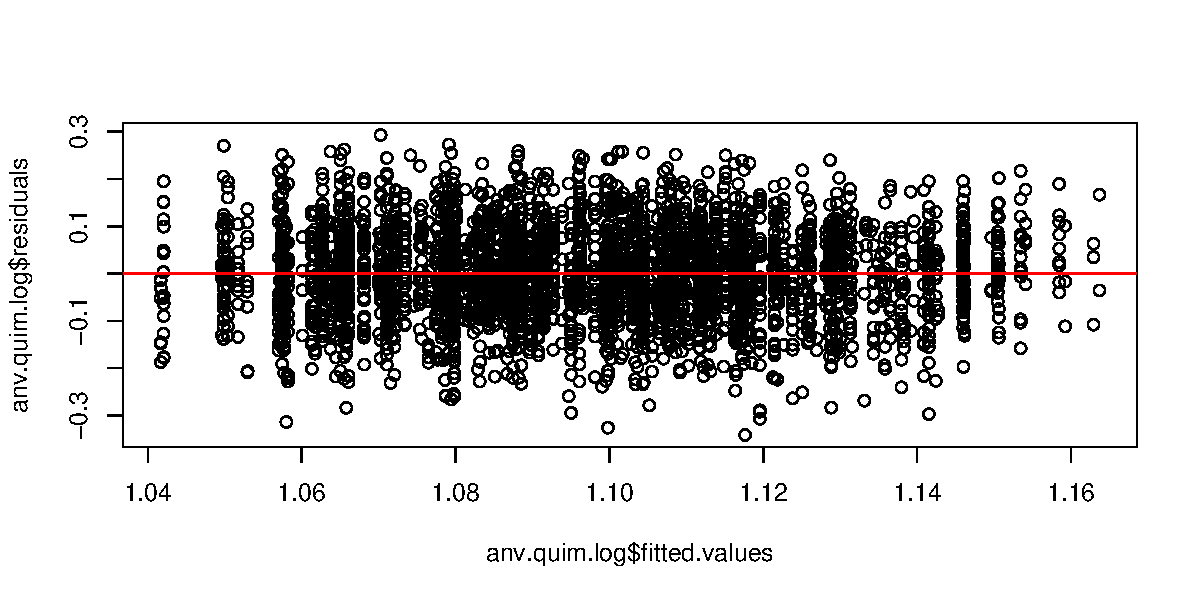
\includegraphics{apresentacao_final_files/figure-beamer/assum_homoc-1} 

}

\caption{Residuals vs Fitted}\label{fig:assum_homoc}
\end{figure}

\end{frame}

\begin{frame}{Validação das premissas \textbar{} Independência}
\protect\hypertarget{validacao-das-premissas-independencia}{}

\begin{itemize}
\tightlist
\item
  Cada execução do processo é independente da outra
\item
  Existem intâncias de diferentes meses e dias, o que garante ainda mais
  a independência
\item
  Pode existir certa dependência se as instâncias forem analisadas de
  forma sequencial. Isso só seria observado dentro de uma mesma turma.
\end{itemize}

\end{frame}

\begin{frame}[fragile]{Resultados}
\protect\hypertarget{resultados}{}

\begin{Shaded}
\begin{Highlighting}[]
\KeywordTok{summary}\NormalTok{(anv.quim.log)}
\end{Highlighting}
\end{Shaded}

\begin{verbatim}
##                  Df Sum Sq Mean Sq F value  Pr(>F)    
## turma             3   0.74 0.24799  27.847 < 2e-16 ***
## material          7   0.10 0.01463   1.642 0.11872    
## mes               9   1.16 0.12895  14.480 < 2e-16 ***
## turma:material   21   0.36 0.01733   1.946 0.00601 ** 
## Residuals      3734  33.25 0.00891                    
## ---
## Signif. codes:  0 '***' 0.001 '**' 0.01 '*' 0.05 '.' 0.1 ' ' 1
\end{verbatim}

\begin{Shaded}
\begin{Highlighting}[]
\KeywordTok{summary.lm}\NormalTok{(anv.quim.log)}\OperatorTok{$}\NormalTok{r.squared}
\end{Highlighting}
\end{Shaded}

\begin{verbatim}
## [1] 0.06655427
\end{verbatim}

\end{frame}

\begin{frame}{Resultados}
\protect\hypertarget{resultados-1}{}

\begin{center}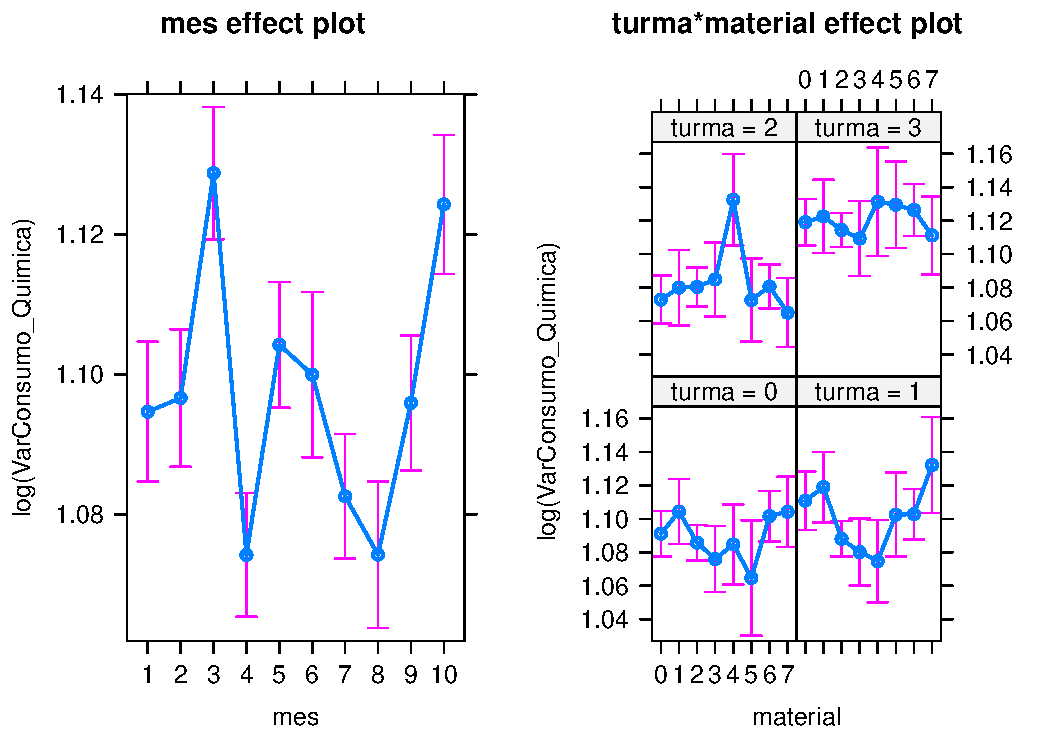
\includegraphics{apresentacao_final_files/figure-beamer/effects_plot_o2-1} \end{center}

\end{frame}

\begin{frame}{Resultados}
\protect\hypertarget{resultados-2}{}

\begin{center}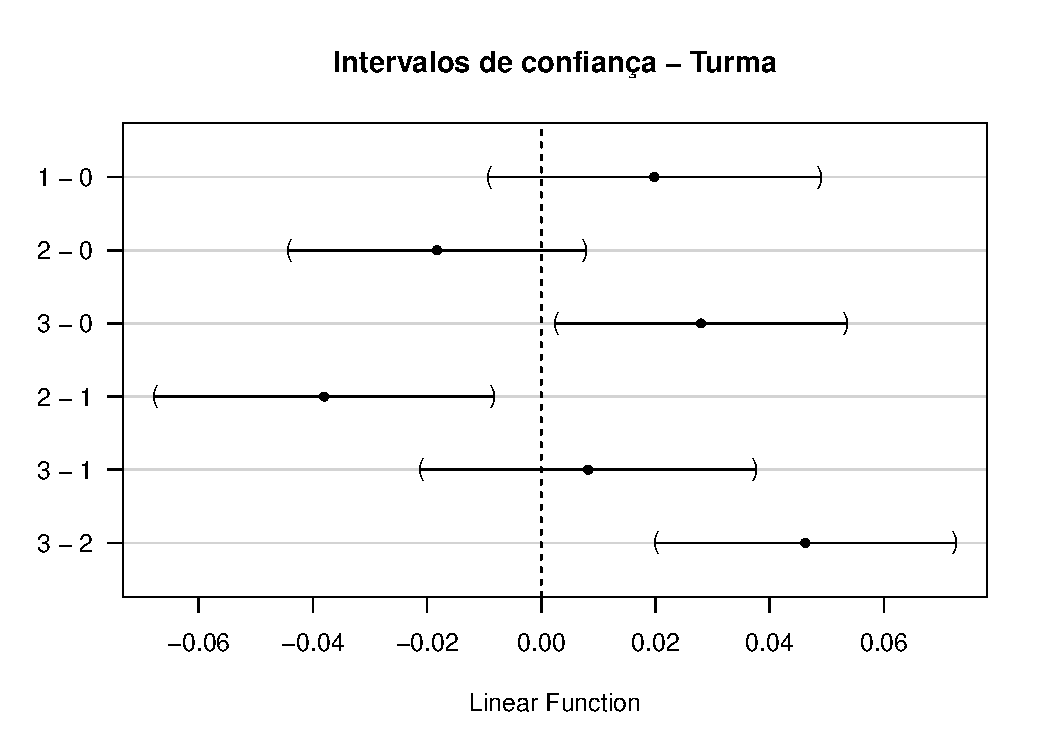
\includegraphics{apresentacao_final_files/figure-beamer/effects_mpc_o2_turma-1} \end{center}

\end{frame}

\begin{frame}{Resultados}
\protect\hypertarget{resultados-3}{}

\begin{center}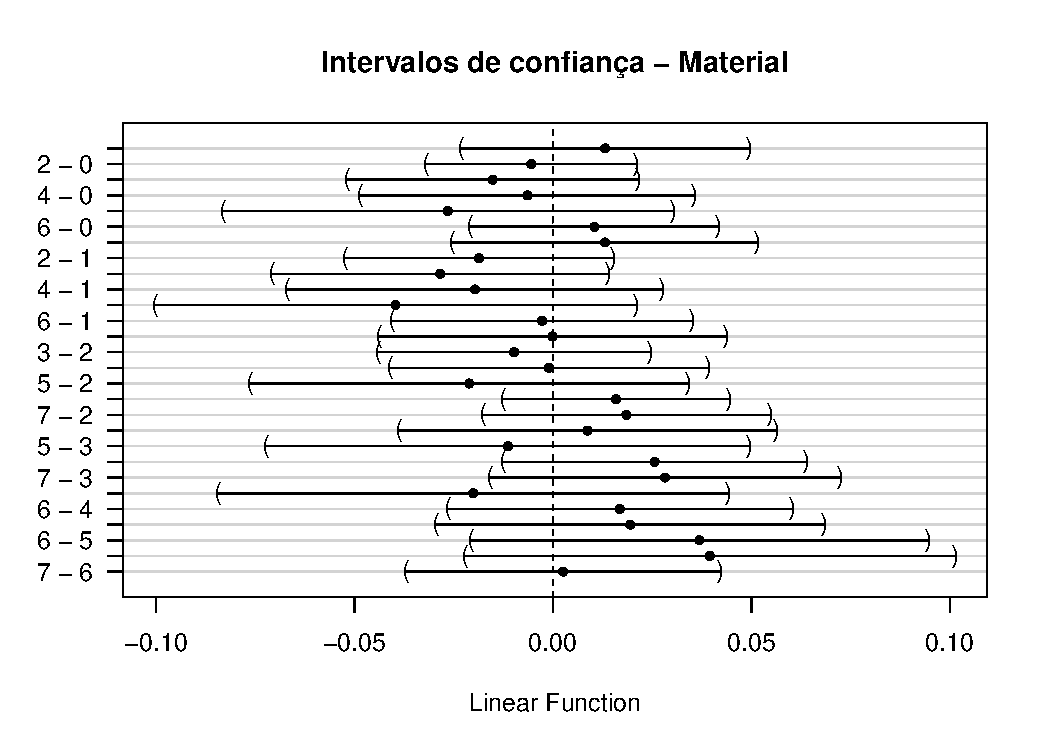
\includegraphics{apresentacao_final_files/figure-beamer/effects_mpc_o2_material-1} \end{center}

\end{frame}

\begin{frame}{Resultados}
\protect\hypertarget{resultados-4}{}

\begin{center}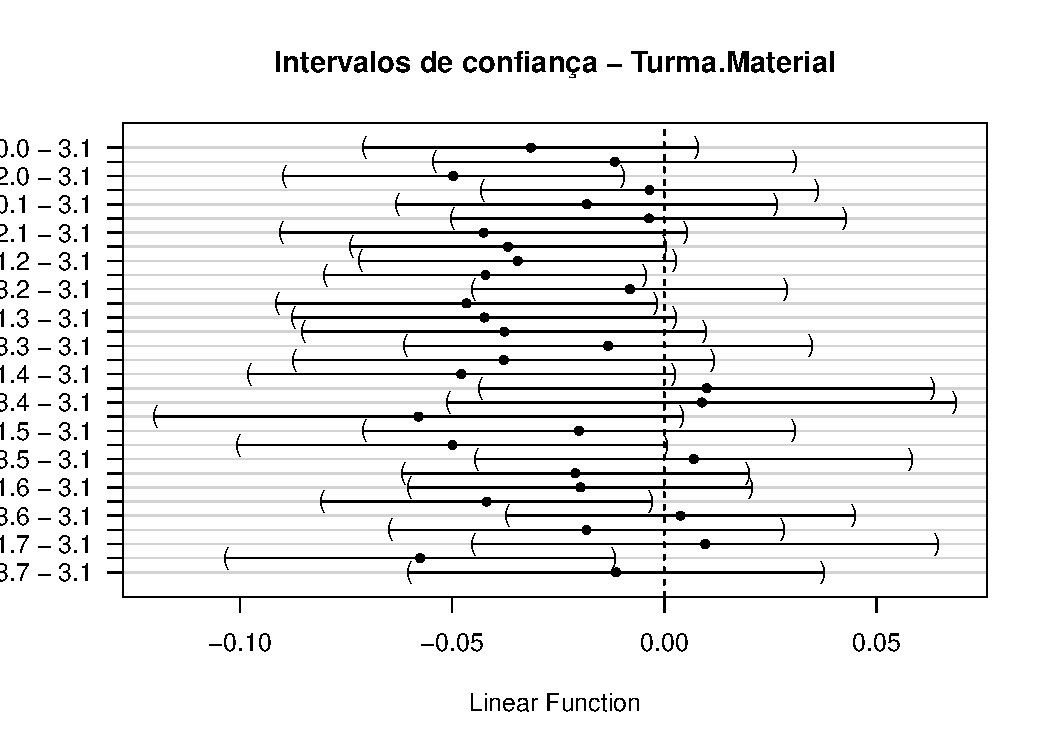
\includegraphics{apresentacao_final_files/figure-beamer/effects_mpc_o2_inter-1} \end{center}

\end{frame}

\begin{frame}{Conclusão}
\protect\hypertarget{conclusao}{}

\begin{itemize}
\tightlist
\item
  O modelo possui um \(R^2\) muito baixo: os fatores turma e material
  sozinhos conseguem explicar 6\% da variância dos dados. Mesmo assim,
  os resultados do ANOVA não deixam de ser significativos, já que não
  estamos interessados na predição do consumo {[}4{]}.
\item
  Não existem diferenças de consumo significativas ao se considerar
  somente o fator material
\item
  A turma 3 possui diferença significativa em relação à 2 e 0, porém o
  mesmo não pode ser concluído para a 1.
\end{itemize}

\end{frame}

\begin{frame}{Referências}
\protect\hypertarget{referencias}{}

\hypertarget{refs}{}
\leavevmode\hypertarget{ref-Montgomery:2006:applied}{}%
{[}1{]} D. C. Montgomery, \emph{Design and analysis of experiments}.
USA: John Wiley \&\#38; Sons, Inc., 2006.

\leavevmode\hypertarget{ref-montgomery2007applied}{}%
{[}2{]} D. C. Montgomery and G. C. Runger, \emph{Applied statistics and
probability for engineers, (with cd)}. John Wiley \& Sons, 2007.

\leavevmode\hypertarget{ref-10.1093ux2fjpepsyux2fjsp004}{}%
{[}3{]} J. A. Durlak, ``How to Select, Calculate, and Interpret Effect
Sizes,'' \emph{Journal of Pediatric Psychology}, vol. 34, no. 9, pp.
917--928, Feb. 2009.

\leavevmode\hypertarget{ref-HowtoInt53:online}{}%
{[}4{]} ``How to interpret a regression model with low r-squared and low
p values.''
\url{https://blog.minitab.com/blog/adventures-in-statistics-2/how-to-interpret-a-regression-model-with-low-r-squared-and-low-p-values}.

\end{frame}

\end{document}
